% Copyright (C) 2012 Shi.Zhan <g.shizhan.g@gmail.com>
%
% Permission is hereby granted, free of charge, to any person obtaining a copy of this software and associated documentation files (the "Software"), to deal in the Software without restriction, including without limitation the rights to use, copy, modify, merge, publish, distribute, sublicense, and/or sell copies of the Software, and to permit persons to whom the Software is furnished to do so, subject to the following conditions:
%
% The above copyright notice and this permission notice shall be included in all copies or substantial portions of the Software.
%
% THE SOFTWARE IS PROVIDED "AS IS", WITHOUT WARRANTY OF ANY KIND, EXPRESS OR IMPLIED, INCLUDING BUT NOT LIMITED TO THE WARRANTIES OF MERCHANTABILITY, FITNESS FOR A PARTICULAR PURPOSE AND NONINFRINGEMENT. IN NO EVENT SHALL THE AUTHORS OR COPYRIGHT HOLDERS BE LIABLE FOR ANY CLAIM, DAMAGES OR OTHER LIABILITY, WHETHER IN AN ACTION OF CONTRACT, TORT OR OTHERWISE, ARISING FROM, OUT OF OR IN CONNECTION WITH THE SOFTWARE OR THE USE OR OTHER DEALINGS IN THE SOFTWARE.
%
% 课程:人机交互技术及应用
% 班级:传播学1001班
% 课时:40学时,2012年秋季1~10周,每周一、三
% 地点:东九楼D212
% 主页:http://code.google.com/p/hci-course/
% 教师:施展 
% 单位:华中科技大学 武汉光电国家实验室
%
\documentclass{beamer}
\usepackage{fontspec,xunicode,xltxtra,beamerthemesplit}
%\usetheme{Hannover} % White background
\usetheme{Berkeley} % Blue background
\setmainfont[
	BoldFont={WenQuanYi Zen Hei},
	ItalicFont={WenQuanYi Micro Hei}
]{WenQuanYi Micro Hei}
\setsansfont[
	BoldFont={WenQuanYi Zen Hei},
	ItalicFont={WenQuanYi Micro Hei}
]{WenQuanYi Micro Hei}

% 中文环境自动换行
\XeTeXlinebreaklocale "zh"
\XeTeXlinebreakskip = 0pt plus 1pt

% 中文环境修正导航栏
\makeatletter
\def\beamer@linkspace#1{
	\begin{pgfpicture}{0pt}{-1.5pt}{#1}{5.5pt}
		\pgfsetfillopacity{0}
		\pgftext[x=0pt,y=-1.5pt]{.}
		\pgftext[x=#1,y=5.5pt]{.}
	\end{pgfpicture}
}
\makeatother

\title{人机交互技术}
\author{施展}
\institute{华中科技大学~武汉光电国家实验室}
\date{\today}
\titlegraphic{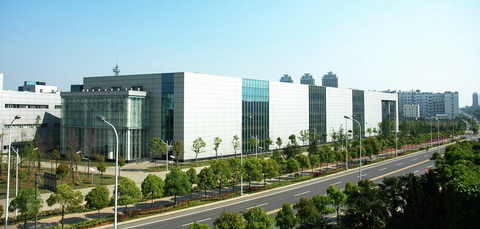
\includegraphics[width=2cm]{images/wnlo.jpg}}

\begin{document}

\begin{frame}
	\titlepage
\end{frame}

\begin{frame}
	\frametitle{内容提要}
	\tableofcontents
\end{frame}

\section{第六讲}
\begin{frame}
	\frametitle{第六讲 人机交互界面表示模型与实现}
	\begin{itemize}
		\item \textbf{目的}: 在界面设计的早期阶段,研究建立一种用户界面表示模型
		\begin{itemize}
			\item 利用形式化的设计语言来分析和表达用户任务以及用户和系统之间的交互情况;
			\item 使界面表示模型能方便地映射到实际的设计实现。
		\end{itemize}
	\end{itemize}
\end{frame}

\begin{frame}
	\frametitle{界面模型分类}
	\begin{itemize}
		\item 任务分解和分析
		\begin{itemize}
			\item 能力模型 Competence Model\\描述用户的目的
			\item 行为模型 Performance Model\\预测和描述用户合法的交互行为序列
		\end{itemize}
		\item 结构模型 Constructional Model\\系统组成模型
	\end{itemize}
\end{frame}

\begin{frame}
	\frametitle{本章主要内容}

\end{frame}

\subsection{人机交互界面表示模型}
\begin{frame}
	\frametitle{{\small 人机交互界面表示模型}~\textbf{行为模型}}

\end{frame}

\subsection{界面描述语言}
\begin{frame}
	\frametitle{界面描述语言}

\end{frame}

\subsection{窗口系统}
\begin{frame}
	\frametitle{窗口系统}

\end{frame}

\subsection{用户界面管理系统}
\begin{frame}
	\frametitle{用户界面管理系统}

\end{frame}

\section{小结}
\begin{frame}
	\frametitle{小结}
	\begin{itemize}
		\item 理解人机交互界面表示模型
		\item 了解窗口系统、用户界面管理系统
	\end{itemize}
\end{frame}

\end{document}